\documentclass[aspectratio=1610]{beamer}

\usetheme{unnslides}
\usefonttheme{professionalfonts}

\usepackage[T2A]{fontenc}
\usepackage[utf8]{inputenc}
\inputencoding{utf8}
\usepackage[russian]{babel}
\usepackage{listings}
\usepackage{graphicx}
\usepackage{caption}
\usepackage{cmbright}
\usepackage{fontspec}
\usepackage{unicode-math}
\usepackage{amsfonts}
\usepackage{subfig}
\usepackage{tikz}

\captionsetup[subfigure]{labelformat=empty}
\captionsetup[figure]{labelformat=empty}

\setmainfont{CMU Sans Serif}
\setromanfont{CMU Sans Serif}
\setsansfont{CMU Sans Serif}

\setlength{\tabcolsep}{1pt}

\usepackage{polyglossia}
\setmainlanguage{russian}
%\setbeamertemplate{itemize item}{\color{black}$\blacktriangleright$}

\DeclareMathOperator*{\argmax}{arg\,max}
\DeclareMathOperator*{\argmin}{arg\,min}
\DeclareMathOperator{\sign}{sign}
\DeclareMathOperator{\re}{Re}

\graphicspath{ {../images/}{img/} }

%set pages numeration
\newcommand\numbered{\setbeamertemplate{footline}{%
  \vspace{-10em}
   \raisebox{5pt}{\makebox[\paperwidth]{%
     \hfill\makebox[10pt]{%
       \usebeamerfont{footline}\usebeamercolor[fg]{footline}
       \insertframenumber}}}}}
\newcommand\unnumbered{\setbeamertemplate{footline}{}}

\title{Параллельный алгоритм для получения равномерного приближения решений множества задач глобальной оптимизации с нелинейными ограничениями}
\author{\underline{\textbf{В.В.~Соврасов}} \and \textbf{К.А.~Баркалов}}
\institute{Нижегородский государственный университет им. Н.И. Лобачевского}
\date{}

\begin{document}
\numbered
{
\unnumbered
\begin{frame}[noframenumbering,plain]
\titlepage
\end{frame}
}

\begin{frame}
  \frametitle{Постановка задачи}
  \begin{columns}
    \begin{column}{0.5\textwidth}
      \begin{displaymath}
        \begin{array}{cr}\\
          \varphi(y^*)=\min\{\varphi(y):y\in D\}, \\
          D=\{y\in \mathbb{R}^N:a_i\leq y_i\leq{b_i}, 1\leq{i}\leq{N},\:g_j(y   )\leqslant 0, 1\leqslant j\leqslant m\}
        \end{array}
      \end{displaymath}
      \(\varphi(y),\:g_j(y)\) -- многоэкстремальные функции, удовлятворяющие условию Липшица:
      \begin{displaymath}
        |f(y_1)-f(y_2)|\leq L\Vert y_1-y_2\Vert,y_1,y_2\in D,
      \end{displaymath}
      где \(L>0\) константа Липшица и \(||\cdot||\) обозначает \(l_2\) норму в пространстве \(\mathbb{R}^N\).
    \end{column}
    \begin{column}{0.5\textwidth}
      \centerline{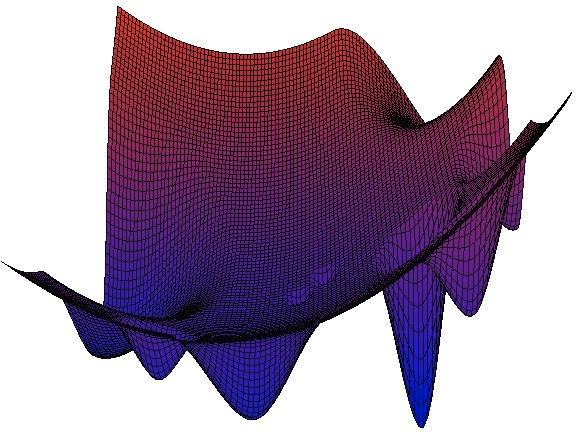
\includegraphics[width=0.9\textwidth]{img/gkls.png}}
    \end{column}
  \end{columns}
\end{frame}

\begin{frame}
  \frametitle{Постановка задачи}
  Далее будем интересоваться решением серии из \(q\) задач глобальной оптимизации с нелинейными ограничениями:
  \begin{displaymath}
    \min\left\{\varphi_1(y), y\in D_1 \right\}, \min\left\{\varphi_2(y), y\in D_2\right\},..., \min\left\{\varphi_q(y), y\in D_q\right\}.
  \end{displaymath}
  Подобные серии задач могут возникнуть, например, в следующих случаях:
  \begin{itemize}
    \item задача глобальной оптимизации с дискретным параметром;
    \item  решение задачи многокритериальной оптимизации методом свертки критериев.
  \end{itemize}
\textbf{Возможные методы решения}:
  \begin{itemize}
    \item решать каждую задачу независимо;
    \item разработать метод оптимизации, который решает все задачи из множества в совокупности, в каждый
    момент времени приоретизируюя одну из них.
  \end{itemize}
\end{frame}

\begin{frame}
  \begin{center}
  \frametitle{Редукция размерноти}
  Кривая Пеано \(y(x)\) позволяет уменьшить размерность многомерного пространства до 1:
  \begin{gather}
    \lbrace y\in \mathbb{R}^N:-2^{-1}\leqslant y_i\leqslant 2^{-1},1\leqslant i\leqslant N\rbrace=\{y(x):0\leqslant x\leqslant 1\} \nonumber \\
    \min\{\varphi(y): y\in D\}=\min\{\varphi(y(x)): x\in [0,1]\} \nonumber
  \end{gather}
  \(y(x)\) является негладкой кривой, отображающей отрезок \([0,1]\) на гиперкуб \(D\).
  \begin{figure}[ht]
    \vspace*{-0.5cm}
    \subfloat{{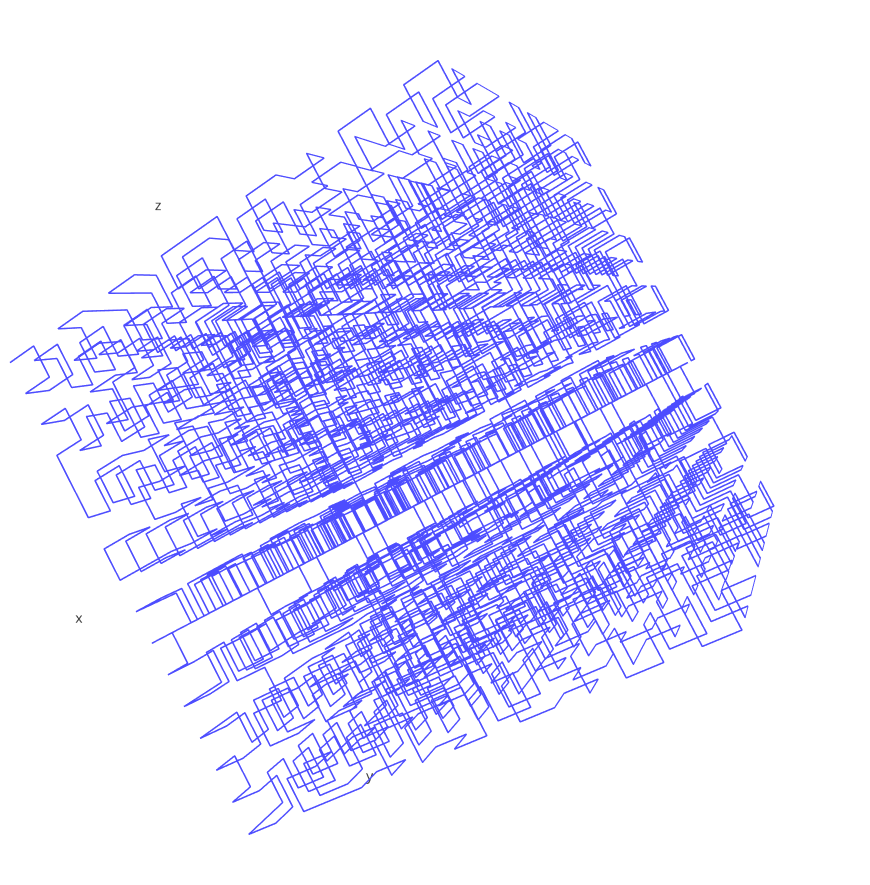
\includegraphics[width=.35\textwidth]{peano3d.png} }}
    \subfloat{{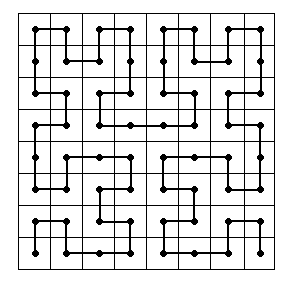
\includegraphics[width=.35\textwidth]{peano2d.png} }}
  \end{figure}
\end{center}
\end{frame}

\begin{frame}
  \frametitle{Алгоритм глобальной оптимизации}
  Метод оптимизации генерирует последовательность точек \(\{x_k:x_k\in[a,b]\}\) и состоит в выполнении следующих шагов:
  \begin{enumerate}
    \setlength{\itemindent}{.1in}
    \item[Шаг 1.] Упорядочить поисковую информацию (одномерные точки) по возрастанию.
    \item[Шаг 2.] Для каждого интервала \((x_{i-1}, x_i)\) вычислить величину \(R(i)\), называемую характеристикой.
    \item[Шаг 3.] Выбрать интервал \((x_{t-1}, x_{t})\) с наибольшей характеристикой и
    провести испытание (вычислить органичения и целевую функцию) в точке \(x^{k+1}\), выбранной с помощью решающего правила \(d\):
    \begin{displaymath}
      x^{k+1}=d(t)\in (x_{t-1}, x_{t})
    \end{displaymath}
    \item[Шаг 4.] Если \(x_{t}-x_{t-1}<\varepsilon\), остановить метод.
  \end{enumerate}
  \textit{\footnotesize	{Детальное описание метода: Strongin R.G., Sergeyev Ya.D.: Global optimization with non-convex constraints. Sequential and parallel algorithms (2000), Chapter 7}}
\end{frame}

\begin{frame}
  \frametitle{Алгоритм, решающий множество задач}
  Создать \(q\) копий характеристического АГО.
  использовать \(q\) синхронно работающих копий ИАГП с тем лишь отличием, что на шаге 6 при выборе
  интервала с наилучшей характеристикой, выбор будет осуществляться из всех интервалов, которые
  породили на данный момент \(q\) копий ИАГП. Если наибольшая характеристика соответствует
  задаче \(i\), то выполняется шаг 7 в копии метода с номером \(i\), а остальные копии метода простаивают.

\end{frame}


\begin{frame}
  \frametitle{Заключение}
    \begin{itemize}
      \item
    \end{itemize}
\end{frame}
{
\unnumbered
\begin{frame}{{}}
  \frametitle{Q\&A}
  \begin{center}
    \Large{Contacts:}
\vspace{0.5cm}

    sovrasov.vlad@gmail.com

    https://github.com/sovrasov
  \end{center}
\end{frame}
}
\end{document}
